\documentclass[12pt]{article}

\usepackage{amsmath}
\usepackage{amsfonts}
\usepackage{float}
\usepackage{fancyhdr}
\usepackage{graphicx}
\usepackage[colorlinks=true,linkcolor=blue, citecolor=red]{hyperref}
\usepackage{url}
\usepackage[top=1.3in, left=1.2in, right=.95in, bottom=1.3in]{geometry}
\usepackage[spanish]{babel}
\usepackage{lipsum}
\usepackage{blindtext}

% For algorithm
\usepackage{algorithm}
\usepackage{algpseudocode}

% ============ CODE ============
\usepackage{listings}
\usepackage{xcolor}
\definecolor{codegreen}{rgb}{0,0.6,0}
\definecolor{codegray}{rgb}{0.5,0.5,0.5}
\definecolor{codepurple}{rgb}{0.58,0,0.82}
\definecolor{backcolour}{rgb}{0.95,0.95,0.92}

% Styling for the code.
\lstdefinestyle{mystyle}{
    backgroundcolor=\color{backcolour},   
    commentstyle=\color{codegreen},
    keywordstyle=\color{magenta},
    numberstyle=\tiny\color{codegray},
    stringstyle=\color{codepurple},
    basicstyle=\ttfamily\footnotesize,
    breakatwhitespace=false,         
    breaklines=true,                 
    captionpos=b,                    
    keepspaces=true,                 
    numbers=left,                    
    numbersep=5pt,                  
    showspaces=false,                
    showstringspaces=false,
    showtabs=false,                  
    tabsize=2
}
\lstset{style=mystyle}

% Disable indentation on new paragraphs
\setlength{\parindent}{0pt}

% Optional: graphic path
% \graphicspath{PATH_TO_GRAPHIC_FOLDER}

% To use Times font family, uncomment this row
% \usepackage{mathptmx}

% To use roman section / subsection, uncomment these rows
% \renewcommand{\thesection}{\Roman{section}}
% \renewcommand{\thesubsection}{\thesection.\Roman{subsection}}

% Define course name, report name and report title.


\newcommand{\coursename}{Escuela Profesional de Ingeniería de Sistemas e Informática} 


%%%%%%INICIO CARATULA%%%%%%%%%%%%%%%%%%%

%informe laboratorio numero
\newcommand{\reportname}{Practica N° 1} 

%titulo del informe
\newcommand{\reporttitle}{Algoritmos de ordenamiento} 

\newcommand{\studentname}{
Nombre y apellido:  \\
{Ricardo Jose Arque Chunga}
}
\newcommand{\teachername}{Honorio Apaza Alanoca}

%\newcommand{\leftfooter}{\LaTeX\ by \href{https://github.com/trhgquan}{Quan, Tran Hoang}}


%%%%%% FIN CARATULA%%%%%%%%%%%%%%%%%%%



% ============ HEADER AND FOOTER ============
% Header length
\setlength{\headheight}{29.43912pt}

% Footer page number would be on the lower-right corner
\pagestyle{fancy}
\fancyfoot{}
\fancyfoot[R]{Pag. \thepage}

\lhead{}
\rhead{
Universidad Nacional de Moquegua\\
\coursename
}
%\lfoot{\leftfooter}

% ============ DOCUMENT ============
\begin{document}
\begin{titlepage}
\newcommand{\HRule}{\rule{\linewidth}{0.5mm}}
\centering

\textsc{\Large \textbf{UNIVERSIDAD NACIONAL DE MOQUEGUA}}\\[0.5cm]
\textsc{\Large Facultad de Ingeniería y Arquitectura }\\[0.5cm]
\textsc{\large Escuela Profesional de Ingeniería de Sistemas e Informática}\\[1.5cm]


\includegraphics[scale=.25]{img/image.png}\\[0.2cm] 

%\textsc{Titulo del trabajo:}\\[0.5cm]

\noindent\hrulefill \\[0.5cm]
{ 
\Large{\bfseries{\reporttitle}}\\[0.5cm]
\large{\bfseries{\reportname}}
}\\[0.4cm]
\noindent\hrulefill \\[0.5cm]

%\textbf{\large Nombres y Apellidos: \coursename}\\[0.5cm]


\begin{minipage}[t]{0.4\textwidth}
\begin{flushleft} \large
\emph{Estudiantes:}\\
\studentname
\end{flushleft}
\end{minipage}
~
\begin{minipage}[t]{0.4\textwidth}
\begin{flushright} \large
\emph{Profesores:} \\
\teachername
\end{flushright}
\end{minipage}\\[2cm]

{\large \today}\\[2cm]



\vfill
\end{titlepage}
	
	
\tableofcontents
\pagebreak

\section{Introducción}
El problema del ordenamiento es uno de los problemas más estudiados en la informática, debido a su relevancia en una amplia gama de aplicaciones y a la complejidad que implica su solución eficiente. El objetivo de un algoritmo de ordenamiento es tomar una secuencia desordenada de elementos y reorganizarlos en un orden predefinido, ya sea ascendente o descendente. En muchos casos, los elementos a ordenar son números, pero también pueden ser cadenas de texto, objetos o cualquier tipo de dato que pueda ser comparado.

El ordenamiento de datos es esencial en muchas áreas de la computación. Por ejemplo, en la búsqueda eficiente de datos, las estructuras de datos como árboles de búsqueda binaria o tablas hash funcionan de manera más efectiva cuando los datos están previamente ordenados. Además, el ordenamiento es un paso crítico en algoritmos de procesamiento de grandes volúmenes de datos, como en la minería de datos, la clasificación de bases de datos y la optimización de consultas en motores de búsqueda.

Existen numerosos algoritmos diseñados para llevar a cabo esta tarea, cada uno con sus características particulares. Estos algoritmos varían en términos de su complejidad temporal, es decir, el tiempo que tardan en ordenar un conjunto de datos, y su complejidad espacial, que mide cuánta memoria adicional se requiere durante el proceso de ordenamiento. Además, los algoritmos de ordenamiento se diferencian en si son estables, lo que significa que mantienen el orden relativo de los elementos con claves iguales, y si son \textit{in situ}, lo que indica que no requieren memoria adicional significativa.

Entre los algoritmos más conocidos se encuentran el \textit{bubblesort}, el \textit{quicksort}, el \textit{mergesort} y el \textit{heapsort}. Cada uno de estos algoritmos tiene sus propias ventajas y desventajas, y su rendimiento depende tanto del tamaño de los datos como de las características del conjunto de datos a ordenar. Por ejemplo, el \textit{bubblesort} es fácil de implementar, pero su complejidad de \(O(n^2)\) lo hace inadecuado para conjuntos grandes de datos. En cambio, el \textit{quicksort} tiene una complejidad promedio de \(O(n \log n)\), lo que lo convierte en uno de los algoritmos más rápidos para la mayoría de los casos prácticos.

Sin embargo, el rendimiento de un algoritmo no solo depende de su complejidad teórica. En la práctica, la eficiencia de un algoritmo también está influenciada por factores como el tipo de entrada y la estructura subyacente de los datos. Algunos algoritmos, como el \textit{quicksort}, son más sensibles al tipo de datos que otros. El \textit{mergesort}, por otro lado, es un algoritmo más robusto en términos de rendimiento, ya que su complejidad \(O(n \log n)\) es garantizada tanto en el peor como en el mejor caso. No obstante, su desventaja es que requiere espacio adicional, lo que puede ser un inconveniente en aplicaciones donde la memoria es limitada.

Por otro lado, el \textit{heapsort}, aunque también tiene una complejidad \(O(n \log n)\), es un algoritmo que no requiere memoria adicional significativa y es especialmente útil en situaciones donde la memoria es un recurso crítico. A pesar de estas ventajas, el \textit{heapsort} tiende a ser más lento en la práctica que otros algoritmos como el \textit{quicksort}, debido a las constantes involucradas en la construcción y manipulación del heap.

\subsection{Importancia Histórica}
Los algoritmos de ordenamiento han jugado un rol clave en el desarrollo de la teoría de la computación desde sus inicios. El estudio de estos algoritmos ha permitido no solo optimizar procesos en sistemas actuales, sino que también ha sido una fuente de inspiración para resolver problemas más complejos en áreas como la inteligencia artificial, la criptografía y el análisis de grandes volúmenes de datos.

\subsection{Optimización en Hardware Moderno}
A medida que el hardware evoluciona, las características de los algoritmos también deben ajustarse para aprovechar al máximo las capacidades de procesamiento paralelo y las arquitecturas de memoria de los sistemas modernos. Por ejemplo, la eficiencia de un algoritmo en una CPU multicore puede diferir de su rendimiento en una GPU, lo que abre nuevas áreas de investigación en el campo de los algoritmos paralelos.

\subsection{Algoritmos Híbridos}
Además de los algoritmos tradicionales, también se han desarrollado algoritmos híbridos, que combinan las mejores características de varios métodos de ordenamiento. Por ejemplo, el algoritmo \textit{Timsort}, utilizado en lenguajes como Python y Java, mezcla \textit{mergesort} e \textit{insertionsort} para mejorar el rendimiento en diferentes tipos de datos.

\subsection{Impacto en la Escalabilidad}
En aplicaciones del mundo real, como sistemas de bases de datos distribuidas o sistemas en la nube, la escalabilidad es un factor crucial. La elección del algoritmo de ordenamiento correcto puede ser la diferencia entre un sistema que escale eficientemente y uno que se vuelva insostenible con grandes volúmenes de datos.

\subsection{Consideraciones en Big Data y Análisis de Datos}
En el contexto de la analítica de datos, donde los conjuntos de datos son masivos y heterogéneos, la elección de un algoritmo de ordenamiento tiene implicaciones significativas en el tiempo de procesamiento y la viabilidad del análisis. Los algoritmos de ordenamiento en este contexto no solo deben ser eficientes, sino que también deben poder manejar entradas distribuidas y procesar datos en \textit{streaming}.


\newpage
\section{Marco teórico}
Los algoritmos de ordenamiento son esenciales en la informática, ya que muchos problemas dependen de la organización eficiente de datos para mejorar su rendimiento y optimización. Estos algoritmos reordenan una secuencia de elementos \( A = \{a_1, a_2, \dots, a_n\} \) para producir una secuencia \( A' = \{a'_1, a'_2, \dots, a'_n\} \), donde \( a'_i \leq a'_j \) para \( 1 \leq i < j \leq n \). A lo largo de los años, se han desarrollado diversos tipos de algoritmos con diferentes propiedades y aplicaciones según el contexto en el que se usen. Los algoritmos analizados en este marco teórico son: \textit{Bubble Sort}, \textit{Counting Sort}, \textit{Heap Sort}, \textit{Insertion Sort}, \textit{Merge Sort}, \textit{Quick Sort}, y \textit{Selection Sort}.

\subsection{Algoritmos de Ordenamiento}

\subsubsection{Bubble Sort}

El \textit{Bubble Sort} es un algoritmo básico de comparación que intercambia elementos adyacentes si están en el orden incorrecto, "burbujeando" los elementos mayores hacia el final de la lista en cada iteración. Aunque es sencillo de entender y fácil de implementar, es uno de los algoritmos más ineficientes para grandes volúmenes de datos debido a su alta complejidad temporal.

\paragraph{Pseudocódigo de Bubble Sort}

\begin{verbatim}
  BubbleSort(A)
  para i desde 1 hasta n-1 hacer
    para j desde 1 hasta n-i hacer
      si A[j] > A[j+1] entonces
        intercambiar A[j] y A[j+1]
\end{verbatim}

\paragraph{Complejidad}

La complejidad temporal de \textit{Bubble Sort} es \( O(n^2) \) tanto en el peor como en el promedio de los casos, ya que el algoritmo requiere realizar múltiples comparaciones e intercambios. En el mejor de los casos, cuando la lista está ordenada, su complejidad es \( O(n) \).

\subsubsection{Counting Sort}

El \textit{Counting Sort} es un algoritmo no comparativo que es particularmente eficiente cuando se ordenan números enteros en un rango acotado. En lugar de comparar los elementos directamente, el algoritmo cuenta cuántas veces aparece cada valor en la lista y utiliza esa información para colocarlos en la posición correcta.

\paragraph{Pseudocódigo de Counting Sort}

\begin{verbatim}
  CountingSort(A, k)
  C[0..k] <- array de ceros
  para j desde 1 hasta n hacer
    C[A[j]] <- C[A[j]] + 1
  para i desde 1 hasta k hacer
    C[i] <- C[i] + C[i-1]
  para j desde n hasta 1 hacer
    B[C[A[j]]] <- A[j]
    C[A[j]] <- C[A[j]] - 1
\end{verbatim}

\paragraph{Complejidad}

El \textit{Counting Sort} tiene una complejidad temporal de \( O(n + k) \), donde \( n \) es el número de elementos a ordenar y \( k \) es el valor máximo en el rango de los datos.

\subsubsection{Heap Sort}

El \textit{Heap Sort} es un algoritmo eficiente basado en la estructura de datos llamada heap (montículo), que puede ser un \textit{max-heap} o un \textit{min-heap}. El \textit{Heap Sort} es un algoritmo in situ que utiliza un heap máximo para ordenar los elementos.

\paragraph{Pseudocódigo de Heap Sort}

\begin{verbatim}
  HeapSort(A)
  construirMaxHeap(A)
  para i desde n hasta 2 hacer
    intercambiar A[1] y A[i]
    n <- n-1
    maxHeapify(A, 1)
\end{verbatim}

\paragraph{Complejidad}

La complejidad temporal de \textit{Heap Sort} es \( O(n \log n) \) en todos los casos.

\subsubsection{Insertion Sort}

El \textit{Insertion Sort} es un algoritmo simple que resulta muy eficiente para listas pequeñas o listas que ya están casi ordenadas. Inserta cada elemento en su posición correcta dentro de la parte ordenada de la lista.

\paragraph{Pseudocódigo de Insertion Sort}

\begin{verbatim}
  InsertionSort(A)
  para i desde 2 hasta n hacer
    clave <- A[i]
    j <- i - 1
    mientras j > 0 y A[j] > clave hacer
      A[j+1] <- A[j]
      j <- j - 1
    A[j+1] <- clave
\end{verbatim}

\paragraph{Complejidad}

El \textit{Insertion Sort} tiene una complejidad temporal de \( O(n^2) \) en el peor de los casos, pero en el mejor de los casos (cuando la lista ya está ordenada), su complejidad es \( O(n) \).

\subsubsection{Merge Sort}

El \textit{Merge Sort} es un algoritmo eficiente que utiliza la técnica de \textit{divide y vencerás}. Divide la lista en dos mitades, las ordena recursivamente y luego combina las dos mitades ordenadas.

\paragraph{Pseudocódigo de Merge Sort}

\begin{verbatim}
  MergeSort(A, p, r)
  si p < r entonces
    q <- (p + r) / 2
    MergeSort(A, p, q)
    MergeSort(A, q+1, r)
    Merge(A, p, q, r)
  
  Merge(A, p, q, r)
  L <- A[p..q]
  R <- A[q+1..r]
  combinar L y R en A[p..r]
\end{verbatim}

\paragraph{Complejidad}

La complejidad temporal del \textit{Merge Sort} es \( O(n \log n) \) en todos los casos.

\subsubsection{Quick Sort}

El \textit{Quick Sort} es uno de los algoritmos más rápidos en la práctica y también sigue la estrategia de \textit{divide y vencerás}. Selecciona un pivote y reordena los elementos en torno a este pivote, de forma que los menores que el pivote queden a su izquierda y los mayores a su derecha.

\paragraph{Pseudocódigo de Quick Sort}

\begin{verbatim}
  QuickSort(A, p, r)
  si p < r entonces
    q <- particionar(A, p, r)
    QuickSort(A, p, q-1)
    QuickSort(A, q+1, r)
  
  Particionar(A, p, r)
  pivote <- A[r]
  i <- p - 1
  para j desde p hasta r-1 hacer
    si A[j] <= pivote entonces
      i <- i + 1
      intercambiar A[i] y A[j]
  intercambiar A[i+1] y A[r]
  retornar i+1
\end{verbatim}

\paragraph{Complejidad}

La complejidad promedio de \textit{Quick Sort} es \( O(n \log n) \), pero en el peor de los casos puede ser \( O(n^2) \).

\subsubsection{Selection Sort}

El \textit{Selection Sort} es un algoritmo que selecciona repetidamente el elemento más pequeño (o más grande) de la lista no ordenada y lo coloca en su posición correcta en la parte ordenada de la lista.

\paragraph{Pseudocódigo de Selection Sort}

\begin{verbatim}
  SelectionSort(A)
  para i desde 1 hasta n-1 hacer
    minIndex <- i
    para j desde i+1 hasta n hacer
      si A[j] < A[minIndex] entonces
        minIndex <- j
    intercambiar A[i] y A[minIndex]
\end{verbatim}

\paragraph{Complejidad}

La complejidad temporal del \textit{Selection Sort} es \( O(n^2) \), tanto en el mejor como en el peor de los casos.
\newpage
\section{Implementacion:}
\subsection{Algoritmos:}
\subsubsection{Bubble Sort}
\begin{verbatim}
import time

ruta = 'archivo.txt'

inicio_tiempo = time.time()

with open(ruta, 'r') as archivo:
    datos = archivo.read()

arreglo = list(map(int, datos.split()))

n = len(arreglo)
for i in range(n):
    for j in range(0, n-i-1):
        if arreglo[j] > arreglo[j+1]:
            arreglo[j], arreglo[j+1] = arreglo[j+1], arreglo[j]

with open(ruta, 'w') as archivo:
    archivo.write(' '.join(map(str, arreglo)))

fin_tiempo = time.time()
print(f"Tiempo de ejecución: {fin_tiempo - inicio_tiempo} segundos")
\end{verbatim}
\subsubsection{Counting Sort}
\begin{verbatim}
import time
ruta = 'archivo.txt'
inicio_tiempo = time.time()
with open(ruta, 'r') as archivo:
    datos = archivo.read()
arreglo = list(map(int, datos.split()))

max_valor = max(arreglo)

conteo = [0] * (max_valor + 1)

for numero in arreglo:
    conteo[numero] += 1

indice = 0
for i in range(len(conteo)):
    while conteo[i] > 0:
        arreglo[indice] = i
        indice += 1
        conteo[i] -= 1

with open(ruta, 'w') as archivo:
    archivo.write(' '.join(map(str, arreglo)))

fin_tiempo = time.time()
print(f"Tiempo de ejecución: {fin_tiempo - inicio_tiempo} segundos")
\end{verbatim}
\subsubsection{Heap Sort}
\begin{verbatim}
import time

ruta = 'archivo.txt'

inicio_tiempo = time.time()

with open(ruta, 'r') as archivo:
    datos = archivo.read()

arreglo = list(map(int, datos.split()))

n = len(arreglo)

for i in range(n // 2 - 1, -1, -1):
    indice = i
    while True:
        hijo_izq = 2 * indice + 1
        hijo_der = 2 * indice + 2
        mayor = indice
        if hijo_izq < n and arreglo[hijo_izq] > arreglo[mayor]:
            mayor = hijo_izq
        if hijo_der < n and arreglo[hijo_der] > arreglo[mayor]:
            mayor = hijo_der
        if mayor == indice:
            break
        arreglo[indice], arreglo[mayor] = arreglo[mayor], arreglo[indice]
        indice = mayor

for i in range(n - 1, 0, -1):
    arreglo[i], arreglo[0] = arreglo[0], arreglo[i]  
    tamaño_heap = i
    indice = 0
    while True:
        hijo_izq = 2 * indice + 1
        hijo_der = 2 * indice + 2
        mayor = indice
        if hijo_izq < tamaño_heap and arreglo[hijo_izq] > arreglo[mayor]:
            mayor = hijo_izq
        if hijo_der < tamaño_heap and arreglo[hijo_der] > arreglo[mayor]:
            mayor = hijo_der
        if mayor == indice:
            break
        arreglo[indice], arreglo[mayor] = arreglo[mayor], arreglo[indice]
        indice = mayor

with open(ruta, 'w') as archivo:
    archivo.write(' '.join(map(str, arreglo)))

fin_tiempo = time.time()
print(f"Tiempo de ejecución: {fin_tiempo - inicio_tiempo} segundos")
\end{verbatim}
\subsubsection{Insertion Sort}
\begin{verbatim}
import time

ruta = 'archivo.txt'

inicio_tiempo = time.time()

with open(ruta, 'r') as archivo:
    datos = archivo.read()

arreglo = list(map(int, datos.split()))

n = len(arreglo)
for i in range(1, n):
    clave = arreglo[i]
    j = i - 1
    while j >= 0 and clave < arreglo[j]:
        arreglo[j + 1] = arreglo[j]
        j -= 1
    arreglo[j + 1] = clave

with open(ruta, 'w') as archivo:
    archivo.write(' '.join(map(str, arreglo)))

fin_tiempo = time.time()
print(f"Tiempo de ejecución: {fin_tiempo - inicio_tiempo} segundos")
\end{verbatim}
\subsubsection{Merge Sort}
\begin{verbatim}
import time

ruta = 'archivo.txt'

inicio_tiempo = time.time()

with open(ruta, 'r') as archivo:
    datos = archivo.read()

arreglo = list(map(int, datos.split()))

n = len(arreglo)
sublistas = [[arreglo[i]] for i in range(n)]

while len(sublistas) > 1:
    nuevas_sublistas = []
    for i in range(0, len(sublistas) - 1, 2):
        izquierda = sublistas[i]
        derecha = sublistas[i + 1]
        temp = []
        while izquierda and derecha:
            if izquierda[0] < derecha[0]:
                temp.append(izquierda.pop(0))
            else:
                temp.append(derecha.pop(0))
        temp += izquierda
        temp += derecha
        nuevas_sublistas.append(temp)
    if len(sublistas) % 2 == 1:
        nuevas_sublistas.append(sublistas[-1])
    sublistas = nuevas_sublistas

arreglo = sublistas[0]

with open(ruta, 'w') as archivo:
    archivo.write(' '.join(map(str, arreglo)))

fin_tiempo = time.time()
print(f"Tiempo de ejecución: {fin_tiempo - inicio_tiempo} segundos")
\end{verbatim}
\subsubsection{Quick Sort}
\begin{verbatim}
import time

ruta = 'archivo.txt'

inicio_tiempo = time.time()

with open(ruta, 'r') as archivo:
    datos = archivo.read()

arreglo = list(map(int, datos.split()))

pila = [(0, len(arreglo) - 1)]

while pila:
    inicio, fin = pila.pop()
    if inicio >= fin:
        continue

    pivote = arreglo[fin]
    i = inicio - 1

    for j in range(inicio, fin):
        if arreglo[j] <= pivote:
            i += 1
            arreglo[i], arreglo[j] = arreglo[j], arreglo[i]

    arreglo[i + 1], arreglo[fin] = arreglo[fin], arreglo[i + 1]
    pivote_index = i + 1

    pila.append((inicio, pivote_index - 1))
    pila.append((pivote_index + 1, fin))

with open(ruta, 'w') as archivo:
    archivo.write(' '.join(map(str, arreglo)))

fin_tiempo = time.time()
print(f"Tiempo de ejecución: {fin_tiempo - inicio_tiempo} segundos")
\end{verbatim}
\subsubsection{Selection Sort}
\begin{verbatim}
import time

ruta = 'archivo.txt'

inicio_tiempo = time.time()

with open(ruta, 'r') as archivo:
    datos = archivo.read()

arreglo = list(map(int, datos.split()))

n = len(arreglo)
for i in range(n):
    min_idx = i
    for j in range(i + 1, n):
        if arreglo[j] < arreglo[min_idx]:
            min_idx = j
    arreglo[i], arreglo[min_idx] = arreglo[min_idx], arreglo[i]

with open(ruta, 'w') as archivo:
    archivo.write(' '.join(map(str, arreglo)))

fin_tiempo = time.time()
print(f"Tiempo de ejecución: {fin_tiempo - inicio_tiempo} segundos")
\end{verbatim}
\subsection{Comparaciones:}
\subsubsection{Por Lenguaje}
\textbf{Python}
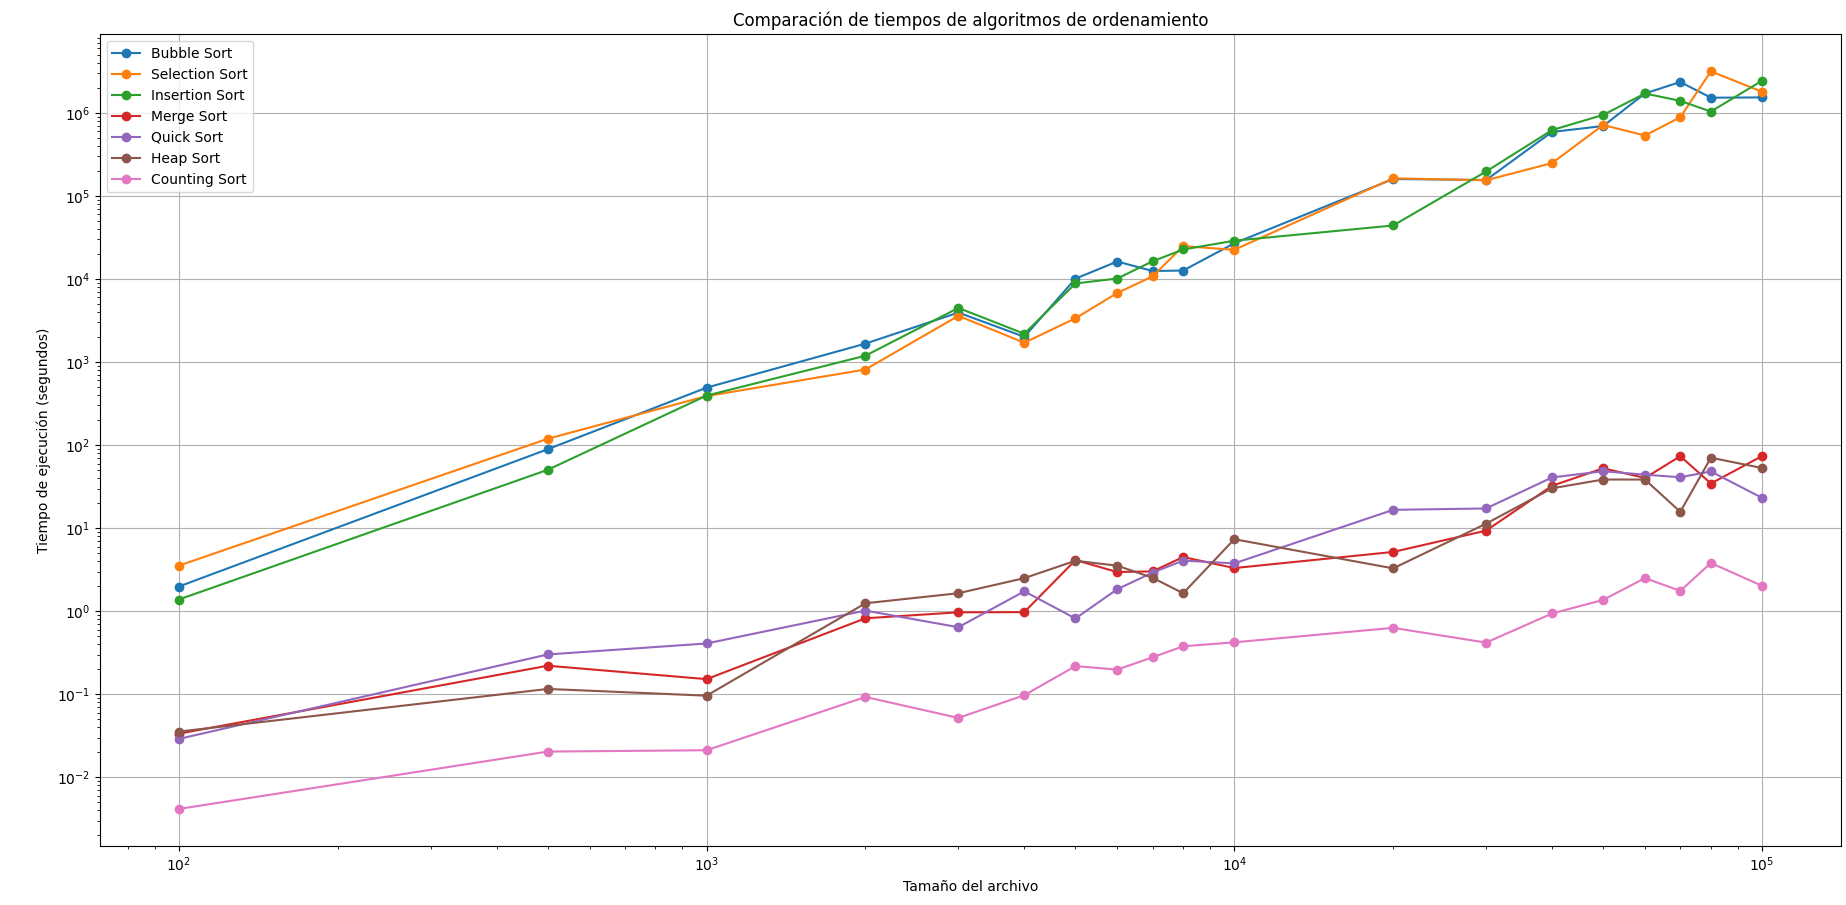
\includegraphics[scale=.25]{img/graficos/por lenguaje/python.png}\\[0.2cm]
\textbf{C++}
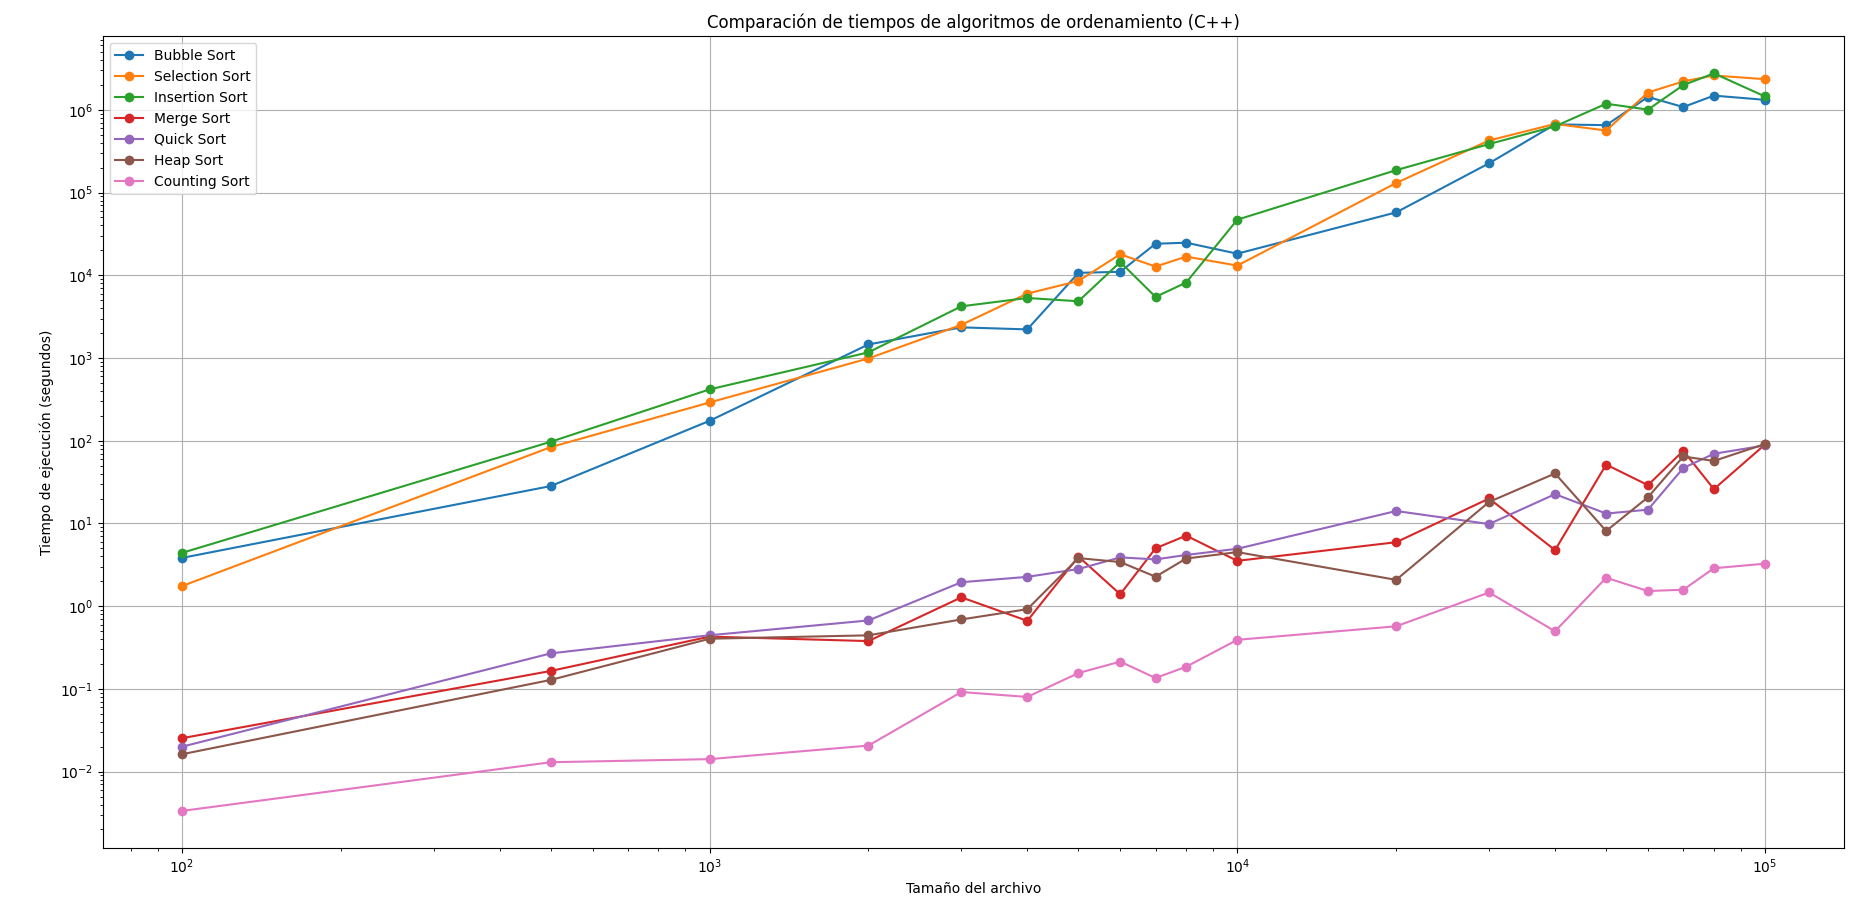
\includegraphics[scale=.25]{img/graficos/por lenguaje/c++.png}\\[0.2cm]
\textbf{JAVA}
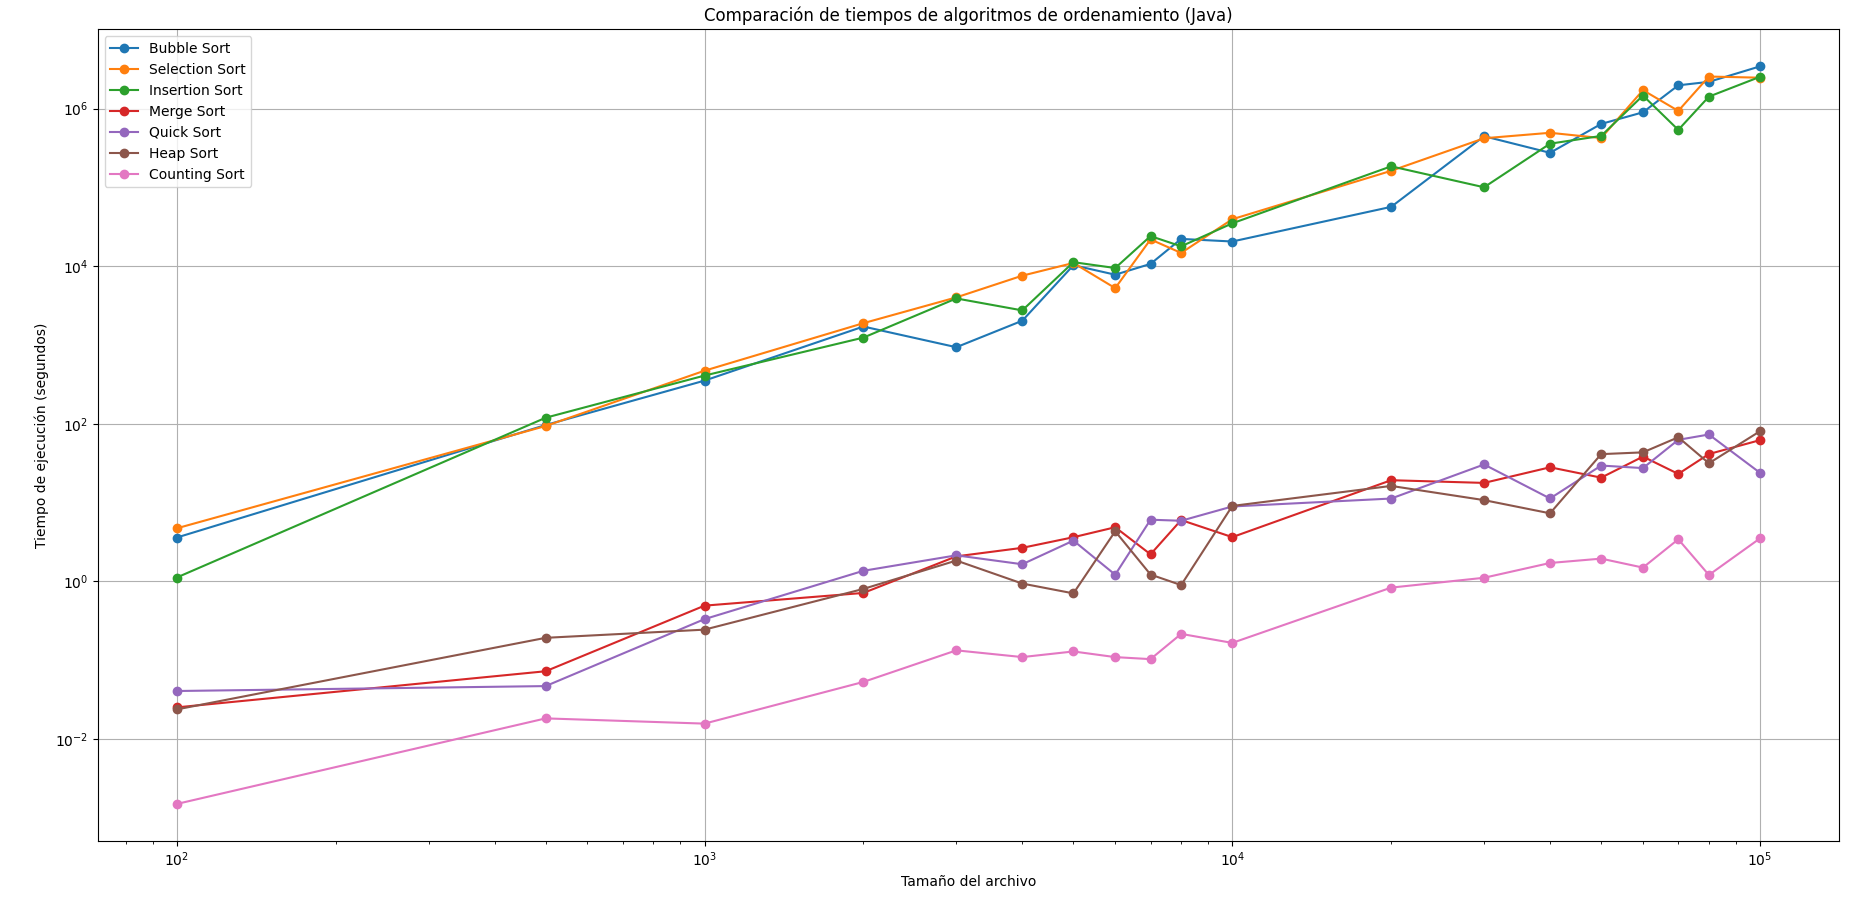
\includegraphics[scale=.25]{img/graficos/por lenguaje/java.png}\\[0.2cm]

\subsubsection{Por Algoritmo}
\textbf{Bubble Sort}
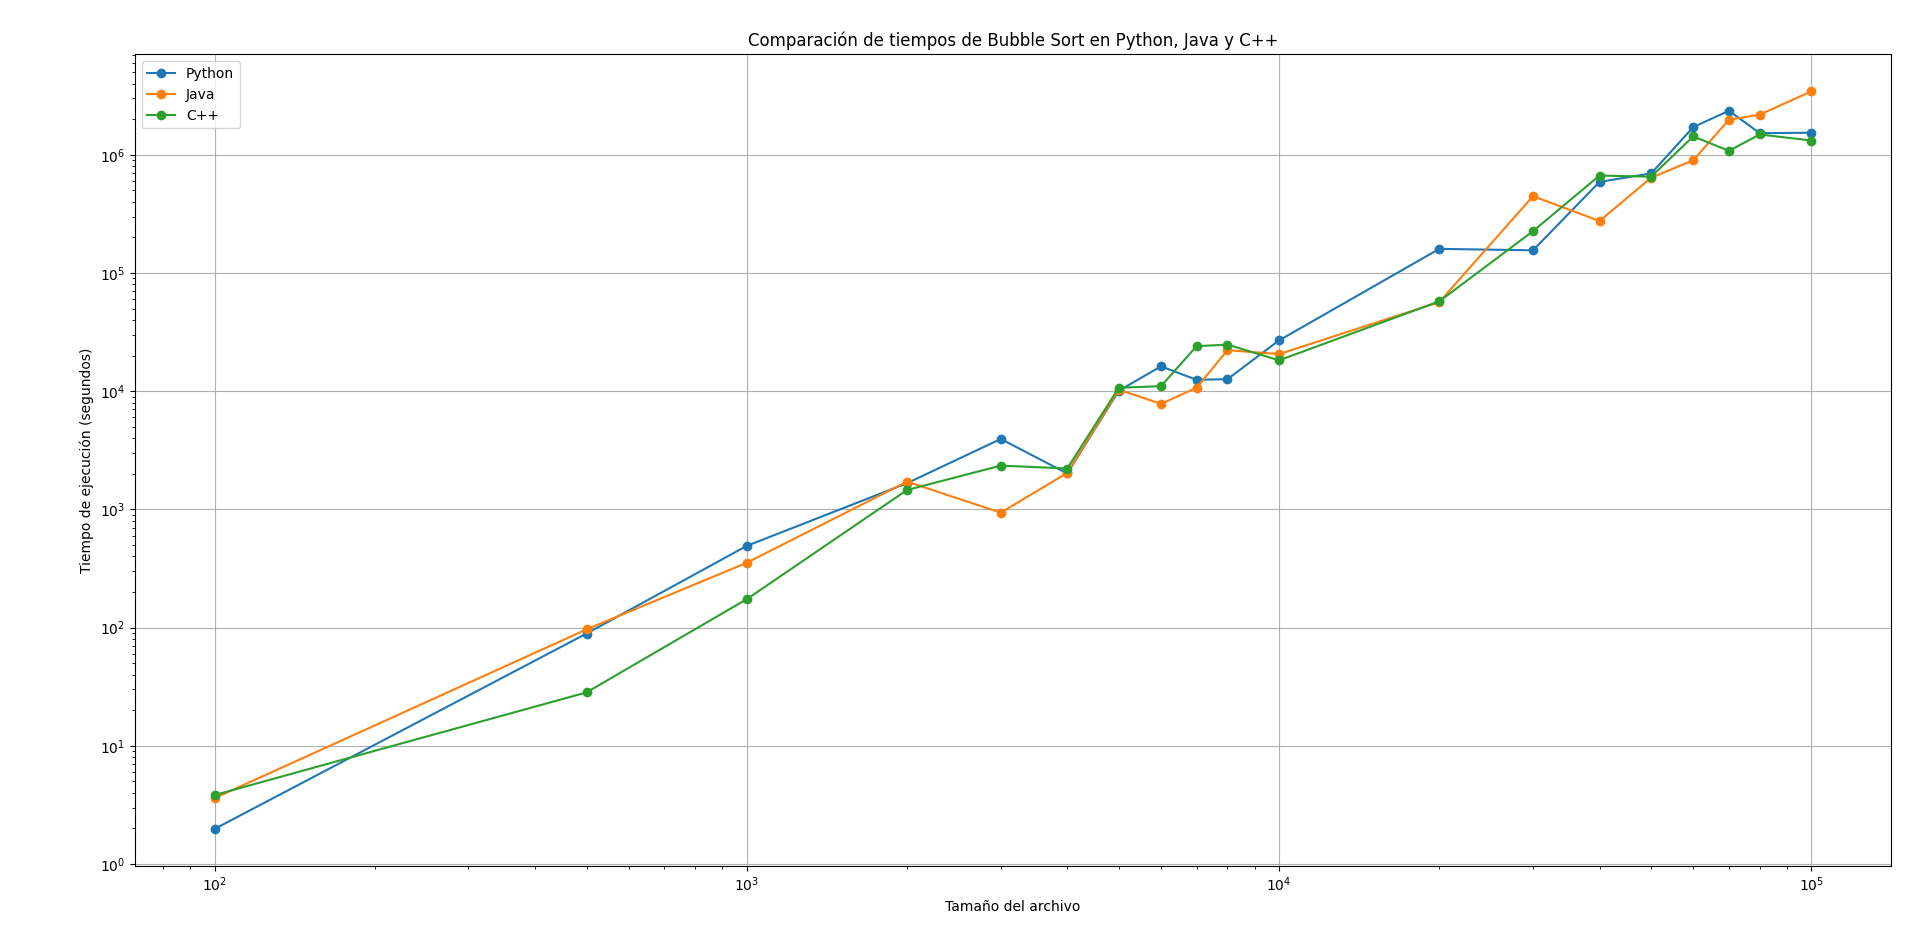
\includegraphics[scale=.25]{img/graficos/por algoritmo/bublesort.png}\\[0.2cm]
\textbf{Counting Sort}
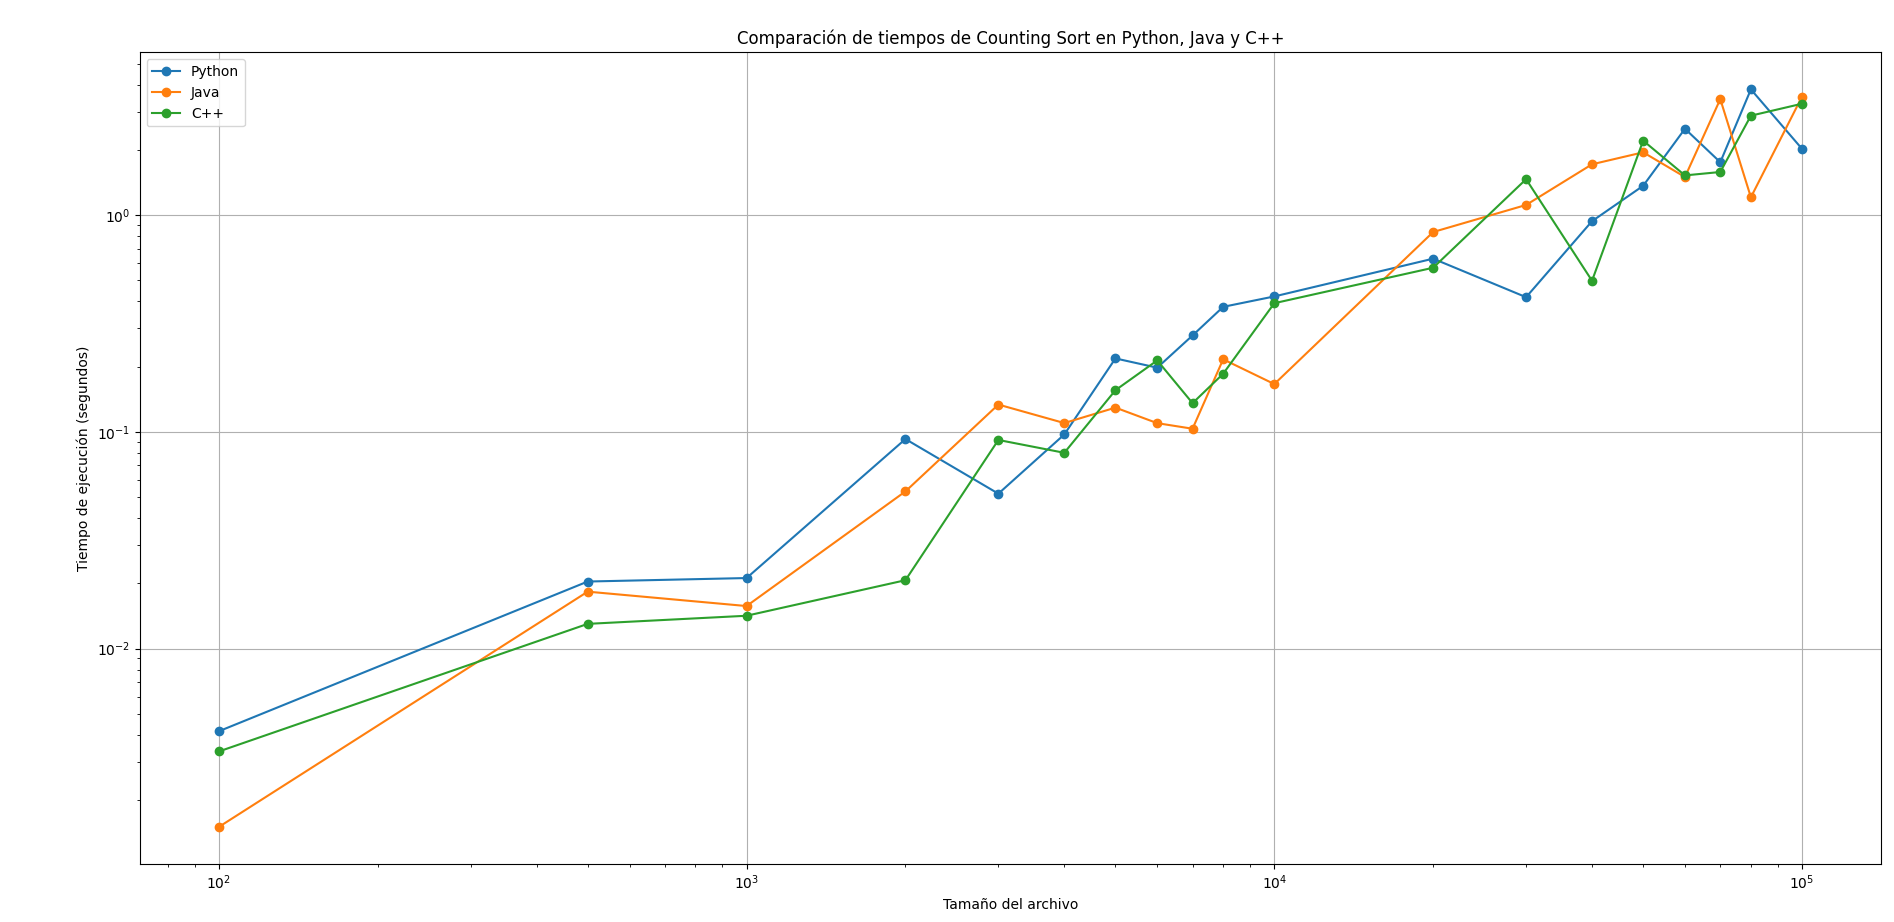
\includegraphics[scale=.25]{img/graficos/por algoritmo/coungtingsort.png}\\[0.2cm]
\textbf{Heap Sort}
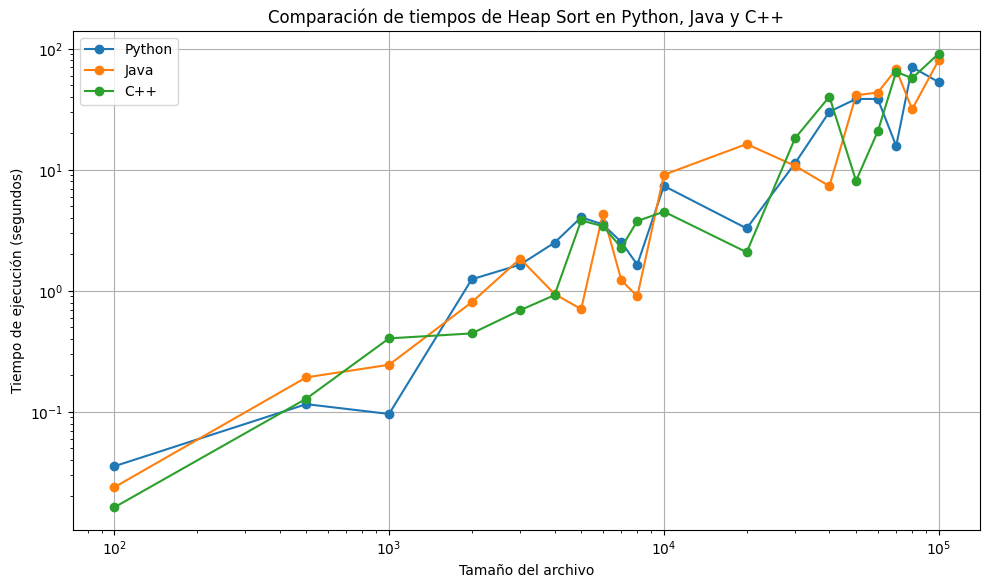
\includegraphics[scale=.25]{img/graficos/por algoritmo/heapsort.png}\\[0.2cm]
\textbf{Insertion Sort}
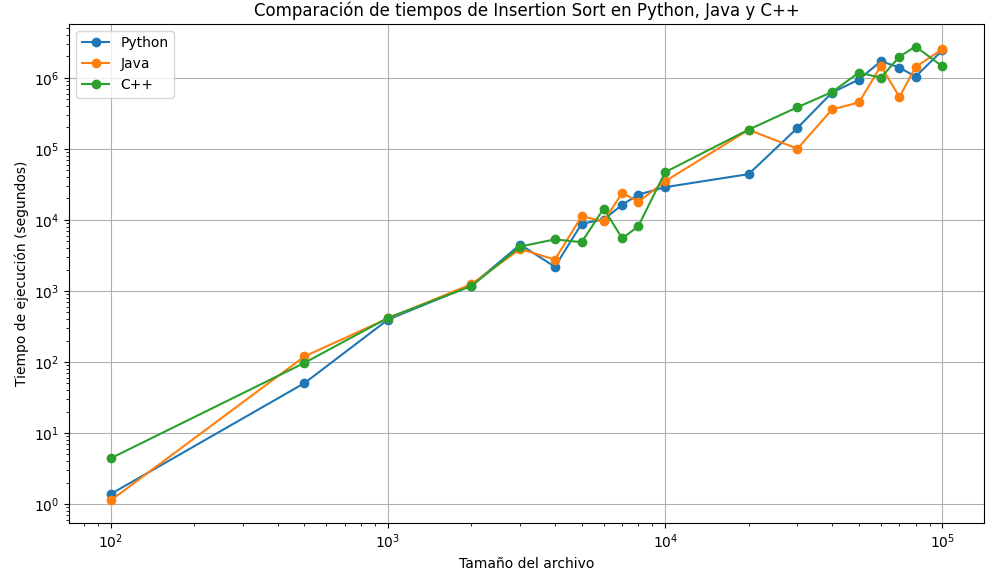
\includegraphics[scale=.25]{img/graficos/por algoritmo/insertionsort.png}\\[0.2cm]
\textbf{Merge Sort}
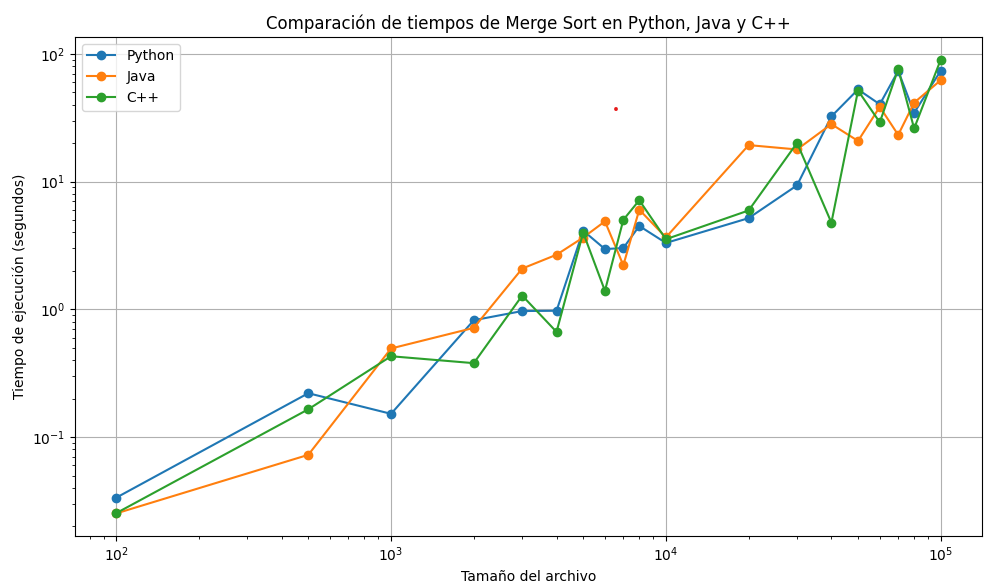
\includegraphics[scale=.25]{img/graficos/por algoritmo/mergersort.png}\\[0.2cm]
\textbf{Quick Sort}
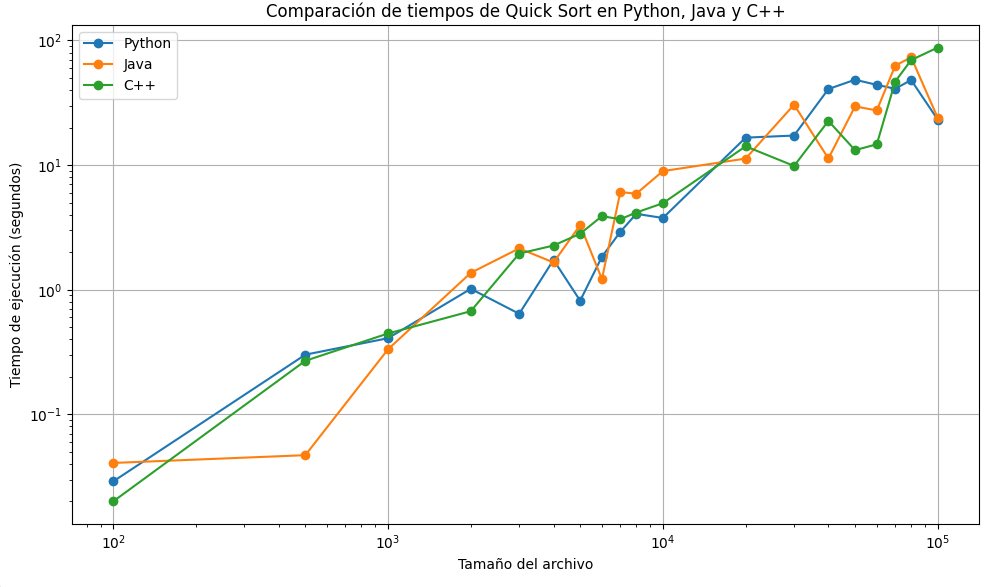
\includegraphics[scale=.25]{img/graficos/por algoritmo/quicksort.png}\\[0.2cm]
\textbf{Selection Sort}
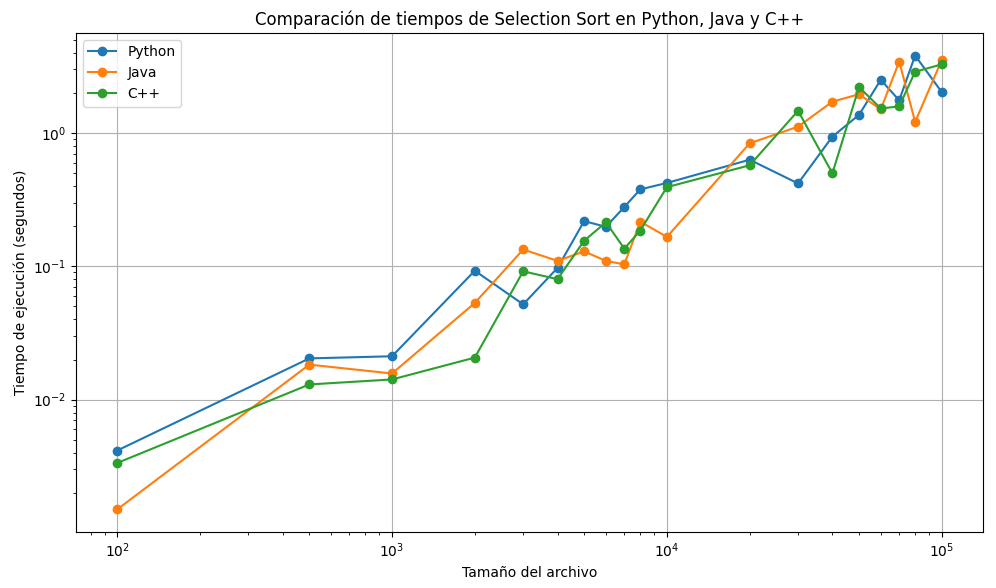
\includegraphics[scale=.25]{img/graficos/por algoritmo/selectionsort.png}\\[0.2cm]
\newpage
\section{Conclusiones}

En este análisis, hemos comparado diferentes algoritmos de ordenamiento implementados en tres lenguajes de programación: \textbf{Python}, \textbf{Java} y \textbf{C++}, observando cómo varían los tiempos de ejecución según el tamaño del archivo y el tipo de algoritmo.

\subsection{Algoritmos Simples: Bubble Sort, Selection Sort, Insertion Sort}
Los algoritmos de ordenamiento básicos como \textbf{Bubble Sort}, \textbf{Selection Sort} e \textbf{Insertion Sort} tienen un desempeño significativamente inferior a medida que aumenta el tamaño de los datos. Esto se debe a su complejidad de tiempo de \(O(n^2)\), lo que provoca que sus tiempos de ejecución crezcan exponencialmente con el tamaño de los archivos.

\begin{itemize}
    \item \textbf{C++} suele ser el lenguaje más eficiente para estos algoritmos debido a su naturaleza compilada y cercana al hardware, mostrando tiempos más bajos en comparación con Python y Java. Esto es especialmente evidente para tamaños de archivo grandes.
    
    \item \textbf{Python}, al ser un lenguaje interpretado, muestra los tiempos de ejecución más altos, reflejando su desventaja en cuanto a eficiencia para estos algoritmos.
    
    \item \textbf{Java}, aunque más eficiente que Python, presenta tiempos de ejecución intermedios. Su compilación en bytecode ofrece ventajas, pero no alcanza la eficiencia de C++.
\end{itemize}

\subsection{Algoritmos más Eficientes: Merge Sort, Quick Sort, Heap Sort}
Los algoritmos más avanzados como \textbf{Merge Sort}, \textbf{Quick Sort} y \textbf{Heap Sort}, con complejidad \(O(n \log n)\), son mucho más eficientes que los algoritmos simples.

\begin{itemize}
    \item \textbf{Quick Sort} muestra un rendimiento consistente en los tres lenguajes, pero en archivos grandes, \textbf{C++} se destaca con tiempos más bajos, seguido de Java y Python.
    
    \item \textbf{Merge Sort} es eficiente en grandes volúmenes de datos, mostrando tiempos competitivos en los tres lenguajes, aunque C++ sigue siendo el más rápido.
    
    \item \textbf{Heap Sort} es menos común pero eficiente, y \textbf{C++} lidera nuevamente en cuanto a tiempos de ejecución.
\end{itemize}

\subsection{Counting Sort: Algoritmo Especializado}
\textbf{Counting Sort}, con complejidad \(O(n+k)\), es extremadamente rápido en los tres lenguajes. En archivos pequeños y medianos, la diferencia entre lenguajes es mínima. Sin embargo, en archivos grandes, \textbf{C++} muestra su eficiencia, seguido de Java y Python.

\subsection{Observaciones Generales sobre los Lenguajes}
\begin{itemize}
    \item \textbf{C++}: Es el lenguaje más eficiente en casi todos los casos, gracias a su naturaleza compilada y su optimización de bajo nivel.
    
    \item \textbf{Java}: Presenta tiempos intermedios, beneficiándose de su compilación en bytecode, pero aún está por debajo de C++ en términos de rendimiento.
    
    \item \textbf{Python}: Es el lenguaje más accesible pero menos eficiente, mostrando tiempos de ejecución significativamente más altos, especialmente en algoritmos de complejidad \(O(n^2)\).
\end{itemize}

\subsection{Conclusión Final}
Los tiempos de ejecución dependen tanto del \textbf{algoritmo} como del \textbf{lenguaje de programación} utilizado. Los algoritmos simples como \textbf{Bubble Sort} e \textbf{Insertion Sort} son ineficientes y muestran grandes diferencias entre lenguajes. Los algoritmos avanzados como \textbf{Quick Sort} y \textbf{Merge Sort} son mucho más eficientes, siendo \textbf{C++} el lenguaje más rápido, seguido de \textbf{Java} y finalmente \textbf{Python}.

Para aplicaciones que requieren alta eficiencia, especialmente con grandes volúmenes de datos, se recomienda usar algoritmos con complejidad \(O(n \log n)\) y considerar \textbf{C++} o \textbf{Java} si el rendimiento es una prioridad.

\end{enumerate}


\end{document}